\section*{Problem No.4} \label{sec:prob4}


\begin{figure}[b]
\centering        
   \subfloat [\emph{mandrill} image] {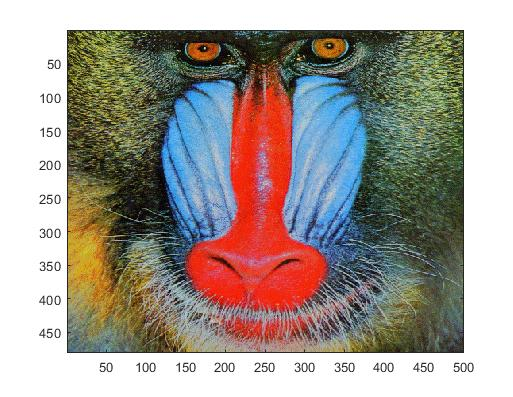
\includegraphics[width=0.5\textwidth]{p4/p4_a.jpg}}
   \subfloat [distribution of singular values]{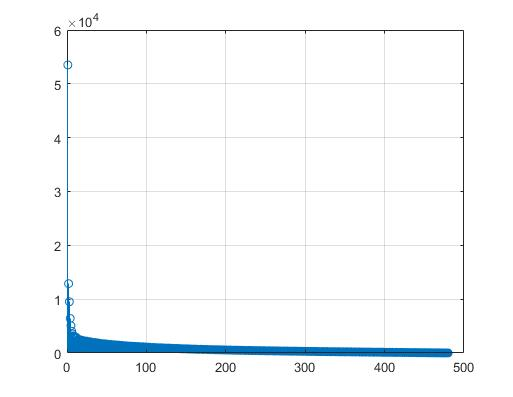
\includegraphics[width=0.5\textwidth]{p4/p4_b.jpg}}
   \caption{ The image (left) along with the distribution of its singular values (right).}
   \label{fig:fig4_ab}
\end{figure}

\begin{figure}[]
\centering        
   \subfloat {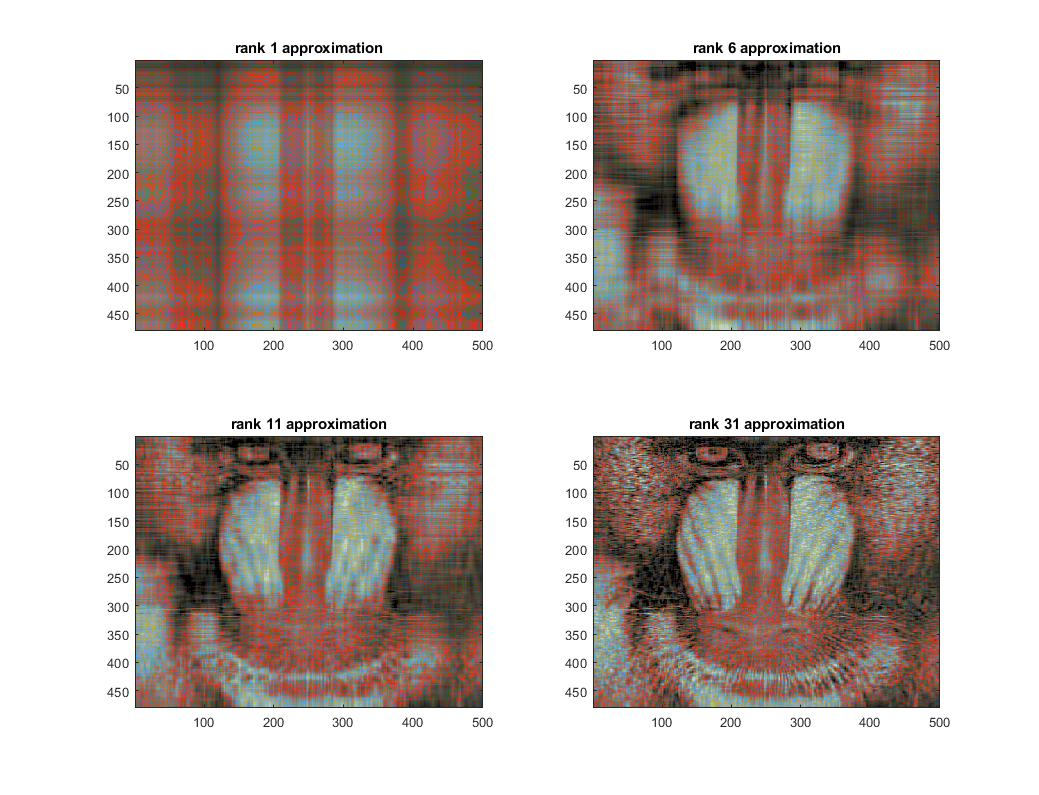
\includegraphics[width=0.95\textwidth]{p4/p4_c.jpg}}
   \caption{Four different approximation for the image based on the rank. }
   \label{fig:fig4_c}
\end{figure}

\begin{figure}[]
 \centering    
\begin{tabular}{ |p{5cm}|| p{3cm}|p{3cm}|}
 \hline
 & Absolute Error &  Relative Error \\ \hhline{|=|=|=|}
 \hline
 Rank 1 approximation  & $12891.1649$ & $1.2699e^{-15}$    \\
 Rank 6 approximation  & $3537.8836$  & $6.4268e^{-16}$   \\
 Rank 11 approximation & $2820.0648$  & $6.4502e^{-16}$   \\
 Rank 31 approximation & $1985.461 $  & $4.5808e^{-16}$   \\
 \hline
\end{tabular} 
\caption{The absolute error (norm) along with relative error of the approximation of  image based of the rank.}
   \label{tab:error}
\end{figure} 